	%%  A simple AAU report template.

%  2014-09-13 v. 1.1.0
%  Copyright 2010-2014 by Jesper Kjær Nielsen <jkn@es.aau.dk>
%
%  This is free software: you can redistribute it and/or modify
%  it under the terms of the GNU General Public License as published by
	%  the Free Software Foundation, either version 3 of the License, or
%  (at your option) any later version.
%
%  This is distributed in the hope that it will be useful,
%  but WITHOUT ANY WARRANTY; without even the implied warranty of
%  MERCHANTABILITY or FITNESS FOR A PARTICULAR PURPOSE.  See the
%  GNU General Public License for more details.
%
%  You can find the GNU General Public License at <http://www.gnu.org/licenses/>.
%
%  A simple AAU report template.
%  2014-09-13 v. 1.1.0
%  Copyright 2010-2014 by Jesper Kjær Nielsen <jkn@es.aau.dk>
%
%  This is free software: you can redistribute it and/or modify
%  it under the terms of the GNU General Public License as published by
%  the Free Software Foundation, either version 3 of the License, or
%  (at your option) any later version.
%
%  This is distributed in the hope that it will be useful,
%  but WITHOUT ANY WARRANTY; without even the implied warranty of
%  MERCHANTABILITY or FITNESS FOR A PARTICULAR PURPOSE.  See the
%  GNU General Public License for more details.
%
%  You can find the GNU General Public License at <http://www.gnu.org/licenses/>.
%
\documentclass[11pt,twoside,a4paper,openright]{report}
%%%%%%%%%%%%%%%%%%%%%%%%%%%%%%%%%%%%%%%%%%%%%%%%
% Language, Encoding and Fonts
% http://en.wikibooks.org/wiki/LaTeX/Internationalization
%%%%%%%%%%%%%%%%%%%%%%%%%%%%%%%%%%%%%%%%%%%%%%%%
% Select encoding of your inputs. Depends on
% your operating system and its default input
% encoding. Typically, you should use
%   Linux  : utf8 (most modern Linux distributions)
%            latin1 
%   Windows: ansinew
%            latin1 (works in most cases)
%   Mac    : applemac
% Notice that you can manually change the input
% encoding of your files by selecting "save as"
% an select the desired input encoding. 
\usepackage[utf8]{inputenc}
% Make latex understand and use the typographic
% rules of the language used in the document.
\usepackage[danish,english]{babel}
% Use the vector font Latin Modern which is going
% to be the default font in latex in the future.
\usepackage{lmodern}
% Choose the font encoding
\usepackage[T1]{fontenc}
% For checkmarks: \cmark and crossmarks: \xmark
\usepackage{pifont}
	\newcommand{\cmark}{\ding{51}}%
	\newcommand{\xmark}{\ding{55}}%
%%%%%%%%%%%%%%%%%%%%%%%%%%%%%%%%%%%%%%%%%%%%%%%%
% Graphics and Tables
% http://en.wikibooks.org/wiki/LaTeX/Importing_Graphics
% http://en.wikibooks.org/wiki/LaTeX/Tables
% http://en.wikibooks.org/wiki/LaTeX/Colors
%%%%%%%%%%%%%%%%%%%%%%%%%%%%%%%%%%%%%%%%%%%%%%%%
% load a colour package
\usepackage[table,dvipsnames]{xcolor}
\definecolor{aaublue}{RGB}{33,26,82}% dark blue
\definecolor{lightGrey}{RGB}{240,240,240}% 
% The standard graphics inclusion package
\usepackage{graphicx}
% Load package to convert eps-files to use as figures
\usepackage{epstopdf}

%\usepackage[dvips,final]{graphicx} 
%\usepackage[dvips]{geometry}
\usepackage{color} %include even if images aren’t in color \usepackage{epsfig}
\usepackage{latexsym}
\usepackage{pstricks}

%\usepackage{epsfig}

% Set up how figure and table captions are displayed
\usepackage{caption}
\captionsetup{%
  font=footnotesize,% set font size to footnotesize
  labelfont=bf % bold label (e.g., Figure 3.2) font
}
\usepackage[section]{placeins} % Figurer overskrider ikke sections
% For subfigures
\usepackage{subcaption}
% Make the standard latex tables look so much better
\usepackage{array,booktabs}
% Enable the use of frames around, e.g., theorems
% The framed package is used in the example environment
\usepackage{framed}

% Afstand mellem listepunkter og tilføjelse af resume funktion til lister: \begin{enumerate}[resume]
\usepackage{enumitem}
\setlist{itemsep=-2pt}

% Tilføjer mulighed for at lave enkelte sider i landskab.
\usepackage{lscape}

\newcounter{listcounter}
%%%%%%%%%%%%%%%%%%%%%%%%%%%%%%%%%%%%%%%%%%%%%%%%
% Mathematics
% http://en.wikibooks.org/wiki/LaTeX/Mathematics
%%%%%%%%%%%%%%%%%%%%%%%%%%%%%%%%%%%%%%%%%%%%%%%%
% Defines new environments such as equation,
% align and split 
\usepackage{amsmath}
% Adds new math symbols
\usepackage{amssymb}
% Use theorems in your document
% The ntheorem package is also used for the example environment
% When using thmmarks, amsmath must be an option as well. Otherwise \eqref doesn't work anymore.
\usepackage[framed,amsmath,thmmarks]{ntheorem}

% Tilføjer \degree symbol
\usepackage{textcomp}
\usepackage{gensymb}

% Fjerner mellemrum efter komma i formler.
%\usepackage{icomma}

% Packages for SI units
\usepackage[binary-units]{siunitx}
% Format SI units as italic in italic texts
\sisetup{detect-all}
\sisetup{per-mode=symbol}


% Argument til amsmath der gør parenteser uden om parenteser pænere ved brug af \right og \left kommandoerne
\delimitershortfall=-1pt

%%%%%%%%%%%%%%%%%%%%%%%%%%%%%%%%%%%%%%%%%%%%%%%%
% Page Layout
% http://en.wikibooks.org/wiki/LaTeX/Page_Layout
%%%%%%%%%%%%%%%%%%%%%%%%%%%%%%%%%%%%%%%%%%%%%%%%
% Change margins, papersize, etc of the document
\usepackage[
  inner=28mm,% left margin on an odd page
  outer=41mm,% right margin on an odd page
  ]{geometry}
% Modify how \chapter, \section, etc. look
% The titlesec package is very configureable
\usepackage[explicit]{titlesec}
%\titleformat*{\section}{\normalfont\Large\bfseries\color{aaublue}}
%\titleformat*{\subsection}{\normalfont\large\bfseries\color{aaublue}}
%\titleformat*{\subsubsection}{\normalfont\normalsize\bfseries\color{aaublue}}
%\titleformat*{\paragraph}{\normalfont\normalsize\bfseries\color{aaublue}}
%\titleformat*{\subparagraph}{\normalfont\normalsize\bfseries\color{aaublue}}
\usepackage{calc}

% Spacing omkring kapiteloverskrift
\titlespacing*{\chapter}{0pt}{40pt}{50pt}



% Overskrift med stort nummer til venstre og titel til højre
%\newlength\chapnumb
%\setlength{\chapnumb}{1.5cm}
%\titleformat{\chapter}[block]
%{\normalfont\bfseries}{}{0pt}
%{\parbox[b]{\chapnumb}{%
	  %\fontsize{2cm}{0}\selectfont\thechapter}%
  %\parbox[b]{\dimexpr\textwidth-\chapnumb\relax}{%
    %\raggedleft%
    %\hfill{\Huge#1}\\
    %\rule{\dimexpr\textwidth-\chapnumb\relax}{.5pt}}}
%\titleformat{name=\chapter,numberless}[block]
%{\normalfont\bfseries}{}{0pt}
	%{\Huge#1}

% Clear empty pages between chapters
\let\origdoublepage\cleardoublepage
\newcommand{\clearemptydoublepage}{%
  \clearpage
  {\pagestyle{empty}\origdoublepage}%
}
\let\cleardoublepage\clearemptydoublepage

% Change the headers and footers
\usepackage{fancyhdr}
\pagestyle{fancy}
\fancyhf{} %delete everything
\renewcommand{\headrulewidth}{0pt} %remove the horizontal line in the header
\fancyhead[RE]{\color{black}\small\nouppercase\leftmark} %even page - chapter title
\fancyhead[LO]{\color{black}\small\nouppercase\rightmark} %uneven page - section title
\fancyhead[LE,RO]{\thepage} %page number on all pages
% Do not stretch the content of a page. Instead,
% insert white space at the bottom of the page
\raggedbottom
% Enable arithmetics with length. Useful when
% typesetting the layout.

\setlength{\headheight}{14pt}

% Raise penalties for bastards
\widowpenalty=10000
\clubpenalty=10000

%%%%%%%%%%%%%%%%%%%%%%%%%%%%%%%%%%%%%%%%%%%%%%%%
% Table of Contents
% http://en.wikibooks.org/wiki/LaTeX/Bibliography_Management
%%%%%%%%%%%%%%%%%%%%%%%%%%%%%%%%%%%%%%%%%%%%%%%%
% Add additional commands for Table of Contents
\usepackage{bookmark}

{\setcounter{tocdepth}{1}}

% Control of space between items in Table of Contents
\usepackage[titles]{tocloft}
\setlength{\cftbeforepartskip}{10pt}
\setlength{\cftbeforechapskip}{4pt}
\setlength{\cftbeforesecskip}{2pt}
%%%%%%%%%%%%%%%%%%%%%%%%%%%%%%%%%%%%%%%%%%%%%%%%
% Bibliography
% http://en.wikibooks.org/wiki/LaTeX/Bibliography_Management
%%%%%%%%%%%%%%%%%%%%%%%%%%%%%%%%%%%%%%%%%%%%%%%%
% Add the \citep{key} command which display a
% reference as [author, year]
\usepackage[square]{natbib}

%%%%%%%%%%%%%%%%%%%%%%%%%%%%%%%%%%%%%%%%%%%%%%%%
% Misc
%%%%%%%%%%%%%%%%%%%%%%%%%%%%%%%%%%%%%%%%%%%%%%%%
% Add bibliography and index to the table of
% contents
\usepackage[nottoc]{tocbibind}
% Add the command \pageref{LastPage} which refers to the
% page number of the last page
\usepackage{lastpage}
\usepackage[
%  disable, %turn off todonotes
  colorinlistoftodos, %enable a coloured square in the list of todos
  textwidth=\marginparwidth, %set the width of the todonotes
  textsize=scriptsize, %size of the text in the todonotes
  ]{todonotes}

% Add command \includepdf to add a whole pdf page to document
\usepackage{pdfpages}


% Add option to easy format directory tree
\usepackage{dirtree}

% String manipulation
\usepackage{xstring,xifthen}

% Tikz package for drawing nice figures
\usepackage{tikz}
\usepackage{schemabloc}
\usetikzlibrary{circuits}


% Package for drawing pretty schematics, without leaving LaTex
\usepackage[american currents, american voltages, european resistors, cute inductors,
american ports]{circuitikz}
\usepackage{tikzscale}

% Code syntax highlight
\usepackage{listings}
\lstset{breaklines=true,
		breakatwhitespace=true,
		commentstyle=\color{ForestGreen},
		numbers=left,
		numberstyle=\tiny\color{black},
		keywordstyle=\color{blue},
		basicstyle=\footnotesize\ttfamily,
        showstringspaces=false,
		}
\renewcommand{\lstlistingname}{Code Snippet}

%%%%%%%%%%%%%%%%%%%%%%%%%%%%%%%%%%%%%%%%%%%%%%%%
% Table environments
% http://en.wikibooks.org/wiki/LaTeX/Tables
%%%%%%%%%%%%%%%%%%%%%%%%%%%%%%%%%%%%%%%%%%%%%%%%
% Better table environments for stuff like table width specifier
\usepackage{tabularx}
\usepackage{multirow}
\usepackage{longtable}
%%%%%%%%%%%%%%%%%%%%%%%%%%%%%%%%%%%%%%%%%%%%%%%%
% Project info and abstract
% chapters\abstract.tex, chapters\projectinfo.tex
%%%%%%%%%%%%%%%%%%%%%%%%%%%%%%%%%%%%%%%%%%%%%%%%
% Loads project info and abstract for use in
% hypersetup
\newcommand{\projectFaculty}{%
\iflanguage{english}{%
Vision, Graphics and Interactive Systems%
}{%
Vision, Grafik og Interaktive Systemer%
}}

\newcommand{\projectGroup}{%
\iflanguage{english}{%
Group 18gr842%
}{%
Gruppe 18gr842%
}}

\newcommand{\projectSemester}{%
P8%
}

\newcommand{\projectType}{%
\iflanguage{english}{%
Project Report%
}{%
Projektrapport%
}}

\newcommand{\projectTitle}{%
\iflanguage{english}{%
Noget med Computer Vision%
}{%
Noget med Computer Vision%
}}

\newcommand{\projectSubtitle}{%
\iflanguage{english}{%
- Subtitle -%
}{%
- Undertitel -%
}}

\newcommand{\projectTheme}{%
\iflanguage{english}{%
Computer Vision%
}{%
Computer Vision%
}}

\newcommand{\projectPeriod}{%
\iflanguage{english}{%
Spring Semester 2018%
}{%
Forårssemester 2018%
}}



\newcommand{\projectParticipants}{%
Marike Koch van den Broek\\
Shagen Djanian\\
Niclas Hjorth Stjernholm
}

\newcommand{\projectSupervisors}{%
Kamal Nasrollahi
}

\newcommand{\projectCopies}{8}

\newcommand{\projectCompletion}{
\iflanguage{english}{%
May 30, 2018%
}{
30. maj 2018%
}}




\newcommand{\projectAbstract}{
%Write the abstract here 
}

\newcommand{\projectSynopsis}{
Synopsis
}

%%%%%%%%%%%%%%%%%%%%%%%%%%%%%%%%%%%%%%%%%%%%%%%%
% Hyperlinks
% http://en.wikibooks.org/wiki/LaTeX/Hyperlinks
%%%%%%%%%%%%%%%%%%%%%%%%%%%%%%%%%%%%%%%%%%%%%%%%
% Enable hyperlinks and insert info into the pdf
% file. Hypperref should be loaded as one of the 
% last packages
\usepackage{hyperref}
\hypersetup{%
	%pdfpagelabels=true,%
	plainpages=false,%
	pdfauthor={\projectGroup, \projectFaculty, \iflanguage{english}{Aalborg University}{Aalborg Universitet}},%
	pdftitle={\projectTitle},%
	pdfsubject={\projectTheme},%
	bookmarksnumbered=true,%
	colorlinks,%
	citecolor=black,%aaublue,%
	filecolor=black,%aaublue,%
	linkcolor=black,%aaublue,% you should probably change this to black before printing
	urlcolor=black,%aaublue,%
	pdfstartview=FitH,%
	bookmarksdepth=2,%
}

% Defines where URLs should break
\def\UrlBreaks{\do\/\do-\do_}
\urlstyle{same}

% Give the possibility to autoformat reference based on distance to the referenced page. Ex. \vpageref{}
\usepackage{varioref}


% Package to warn about missing references.
%\usepackage{refcheck}

% Package to make a glossary of acronyms.
\usepackage{glossaries}
\glstoctrue
\makenoidxglossaries
% Glossaries package
% http://ctan.cs.uu.nl/macros/latex/contrib/glossaries/glossariesbegin.pdf
%
% % % % % % % %
%	Example of glossary entry:
% \newglossaryentry{cabbage}{name={cabbage},description={vegetable with thick green or purple leaves}}
%
%	Example of acronym entry:
% \newacronym{spi}{SPI}{Serial Peripheral Interface}
%
% \gls{key}

\newacronym{cdf}{CDF}{Cumulative Distribution Function}
\newacronym{cnn}{CNN}{Convolutional Neural Network}
\newacronym{cpu}{CPU}{Central Processing Unit}
\newacronym{fcn}{FCN}{Fully Convolutional Network}
\newacronym{dbn}{DBN}{Deep Belief Network}
\newacronym{deepid}{DeepID}{Deep hidden identity features}
\newacronym{deepid2}{DeepID2}{Deep IDentification-verification features}
\newacronym{gpu}{GPU}{Graphics Processing Unit}
\newacronym{spdnn}{SPDNN}{Semi Parallel Deep Neural Networks}
\newacronym{lfw}{LFW}{Labeled Faces in the Wild}
\newacronym{hmm}{HMM}{Hidden Markov Model}
\newacronym{lda}{LDA}{Linear Discriminant Analysis}
\newacronym{pca}{PCA}{Principal Component Analysis}
\newacronym{svm}{SVM}{support vector machines}
\newacronym{knn}{KNN}{K-Nearest-Neighbours}
\newacronym{vl}{VL}{Visible Light}
\newacronym{nir}{NIR}{Near Infra-Red}
\newacronym{mcs}{MCS}{Multiple Classifier Systems}
\newacronym{relu}{ReLU}{Rectified Linear Unit}
\newacronym{fc}{FC}{Fully Connected}


% Package to make semi-bold font.
\usepackage[outline]{contour}
\contourlength{0.1pt}
\contournumber{50}%
\newcommand{\textsb}[1]{\contour{black}{#1}}

% Package for splitting lists or other things up in columns. Ex: \begin{multicols}{2}
\usepackage{multicol}

% Package for rotating a page to landscape orientation. Ex: \begin{landscape}
\usepackage{pdflscape}

% Package for circuit diagrams in tikz
\usepackage{circuitikz}

% For adding notes to tables
\usepackage{threeparttable}

% For adding smileys ;) I know....
\usepackage{MnSymbol,wasysym}

% For adding algorithms
\usepackage{algorithm}
\usepackage[noend]{algpseudocode}
\makeatletter
\def\BState{\State\hskip-\ALG@thistlm}
\makeatother

\renewcommand*{\glsgroupskip}{\vspace{2mm}}

% Package to use fixme fxnote
\usepackage[footnote,marginclue,draft,danish,silent,nomargin]{fixme} 

% Package inclusion and set up of the document

% see, e.g., http://en.wikibooks.org/wiki/LaTeX/Formatting#Hyphenation
% for more information on word hyphenation
\hyphenation{ex-am-ple hy-phen-a-tion short}
\hyphenation{long la-tex}
\hyphenation{AAU-Sat}
\hyphenation{minimum-spændinger}
\hyphenation{ud-vik-lings-poten-tiale}
\hyphenation{pick-up pick-up-pen gui-tar-pick-up gui-tar-pick-up-pen pick-uppens}
\hyphenation{tech-no-lo-gy}
\hyphenation{Hø-re-for-e-ning-en}% Hypenation setup

%  A simple AAU report template.
%  2014-09-13 v. 1.1.0
%  Copyright 2010-2014 by Jesper Kjær Nielsen <jkn@es.aau.dk>
%
%  This is free software: you can redistribute it and/or modify
%  it under the terms of the GNU General Public License as published by
%  the Free Software Foundation, either version 3 of the License, or
%  (at your option) any later version.
%
%  This is distributed in the hope that it will be useful,
%  but WITHOUT ANY WARRANTY; without even the implied warranty of
%  MERCHANTABILITY or FITNESS FOR A PARTICULAR PURPOSE.  See the
%  GNU General Public License for more details.
%
%  You can find the GNU General Public License at <http://www.gnu.org/licenses/>.
%
%
%
% see, e.g., http://en.wikibooks.org/wiki/LaTeX/Customizing_LaTeX#New_commands
% for more information on how to create macros

%%%%%%%%%%%%%%%%%%%%%%%%%%%%%%%%%%%%%%%%%%%%%%%%
% Loads user defined variables
%%%%%%%%%%%%%%%%%%%%%%%%%%%%%%%%%%%%%%%%%%%%%%%%

\newcommand{\noSIunit}{$1$}% Definerer hvad der skal skrives hvis symbolet ikke har nogen enhed.
\newcommand{\obcTransducerAddress}{0xB1}% CAN adresse til tranducer modulet i OBC.

\def\circuitScale{.5}%

%%%%%%%%%%%%%%%%%%%%%%%%%%%%%%%%%%%%%%%%%%%%%%%%
% Macros for the titlepage
%%%%%%%%%%%%%%%%%%%%%%%%%%%%%%%%%%%%%%%%%%%%%%%%
%Creates the aau titlepage
\newcommand{\aautitlepage}[3]{%
  {
    %set up various length
    \ifx\titlepageleftcolumnwidth\undefined
      \newlength{\titlepageleftcolumnwidth}
      \newlength{\titlepagerightcolumnwidth}
    \fi
    \setlength{\titlepageleftcolumnwidth}{0.5\textwidth-\tabcolsep}
    \setlength{\titlepagerightcolumnwidth}{\textwidth-2\tabcolsep-\titlepageleftcolumnwidth}
    %create title page
    \thispagestyle{empty}
    \noindent%
    \begin{tabular}{@{}ll@{}}
      \parbox{\titlepageleftcolumnwidth}{
        \iflanguage{danish}{%
          
\includegraphics[page=1,width=\titlepageleftcolumnwidth]{figures/aau_logo}
        }{%
          
\includegraphics[page=2,width=\titlepageleftcolumnwidth]{figures/aau_logo}
        }
      } &
      \parbox{\titlepagerightcolumnwidth}{\raggedleft\sf\small
        #2
      }\bigskip\\
       #1 &
      \parbox[t]{\titlepagerightcolumnwidth}{%
        \iflanguage{danish}{%
          \textbf{Synopsis:}\smallskip\par
        }{%
          \textbf{Abstract:}\smallskip\par
        }
        \fbox{\parbox{\titlepagerightcolumnwidth-2\fboxsep-2\fboxrule}{%
          #3
        }}
      }\\
    \end{tabular}
    \vfill
    \iflanguage{danish}{%
      \noindent{\footnotesize\emph{Rapportens indhold er frit tilgængeligt, men offentliggørelse (med kildeangivelse) må kun ske efter aftale med forfatterne.}}
    }{%
      \noindent{\footnotesize\emph{The content of this report is freely available, but publication may only be pursued with reference.}}
    }
    \cleardoublepage
  }
}

%Create english project info
\newcommand{\englishprojectinfo}[8]{%
  \parbox[t]{\titlepageleftcolumnwidth}{
    \textbf{Title:}\\ #1\bigskip\par
    \textbf{Theme:}\\ #2\bigskip\par
    \textbf{Project Period:}\\ #3\bigskip\par
    \textbf{Project Group:}\\ #4\bigskip\par
    \textbf{Participants:}\\ #5\bigskip\par
    \textbf{Supervisor:}\\ #6\bigskip\par
    \textbf{Number of Pages:} \pageref{LastPage}\bigskip\par
    \textbf{Date of Completion:}\\ #8
  }
}

%Create danish project info
\newcommand{\danishprojectinfo}[8]{%
  \parbox[t]{\titlepageleftcolumnwidth}{
    \textbf{Titel:}\\ #1\bigskip\par
    \textbf{Tema:}\\ #2\bigskip\par
    \textbf{Projektperiode:}\\ #3\bigskip\par
    \textbf{Projektgruppe:}\\ #4\bigskip\par
    \textbf{Deltagere:}\\ #5\bigskip\par
    \textbf{Vejleder:}\\ #6\bigskip\par
    \textbf{Oplagstal:} #7\bigskip\par
    \textbf{Sidetal:} \pageref{LastPage}\bigskip\par
    \textbf{Afleveringsdato:}\\ #8
  }
}

%%%%%%%%%%%%%%%%%%%%%%%%%%%%%%%%%%%%%%%%%%%%%%%%
% An example environment
%%%%%%%%%%%%%%%%%%%%%%%%%%%%%%%%%%%%%%%%%%%%%%%%
\theoremheaderfont{\normalfont\bfseries}
\theorembodyfont{\normalfont}
\theoremstyle{break}
\def\theoremframecommand{{\color{aaublue!50}\vrule width 5pt \hspace{5pt}}}
\newshadedtheorem{exa}{Example}[chapter]
\newenvironment{example}[1]{%
		\begin{exa}[#1]
}{%
		\end{exa}
}


%%%%%%%%%%%%%%%%%%%%%%%%%%%%%%%%%%%%%%%%%%%%%%%%%
% Exponential function defined as upright e, \exp
%%%%%%%%%%%%%%%%%%%%%%%%%%%%%%%%%%%%%%%%%%%%%%%%%
\renewcommand{\exp}{\text{e}}


%%%%%%%%%%%%%%%%%%%%%%%%%%%%%%%%%%%%%%%%%%%%%%%%%%%
% Command \clearevenpage start chapter on even page
%%%%%%%%%%%%%%%%%%%%%%%%%%%%%%%%%%%%%%%%%%%%%%%%%%%
\makeatletter
\newcommand*{\clearevenpage}{%
  \clearpage
  \if@twoside
    \ifodd\c@page
      \hbox{}%
      \newpage
      \if@twocolumn
        \hbox{}%
        \newpage
      \fi
    \fi
  \fi
}
\makeatother

%%%%%%%%%%%%%%%%%%%%%%%%%%%%%%%%%%%%%%%%%%%%%%%%%%%%%%%
% Command \addunit. Use it to add si units to equations
%%%%%%%%%%%%%%%%%%%%%%%%%%%%%%%%%%%%%%%%%%%%%%%%%%%%%%%
\makeatletter
\providecommand\add@text{}
\newcommand\addunit[1]{%
  \gdef\add@text{\text{[}\ifthenelse{\equal{#1}{}}{\noSIunit}{\si{#1}}\text{]}\gdef\add@text{}}}% 
\renewcommand\tagform@[1]{%
  \maketag@@@{\llap{\add@text\quad}(\ignorespaces#1\unskip\@@italiccorr)}%
}
\makeatother

%%%%%%%%%%%%%%%%%%%%%%%%%%%%%%%%%%%%%%%%%%%%%
% Oversættelser af ord ved brug af \autoref{}
%%%%%%%%%%%%%%%%%%%%%%%%%%%%%%%%%%%%%%%%%%%%%
\addto\extrasdanish{%
  \def\figureautorefname{Figur}%
  \def\subfigureautorefname{Figur}%
  \def\tableautorefname{Tabel}%
  \def\partautorefname{Del}%
  \def\appendixautorefname{Bilag}%
  \def\equationautorefname{Ligning}%
  \def\Itemautorefname{Punkt}%
  \def\chapterautorefname{Kapitel}%
  \def\sectionautorefname{Afsnit}%
  \def\subsectionautorefname{Afsnit}%
  \def\subsubsectionautorefname{Underafsnit}%
  \def\paragraphautorefname{Delafsnit}%
  \def\Hfootnoteautorefname{Fodnote}%
  \def\AMSautorefname{Ligning}%
  \def\theoremautorefname{Sætning}%
  \def\pageautorefname{Side}%
  \def\requirementautorefname{Krav}%
}

\addto\extrasenglish{%
  \def\sectionautorefname{section}%
  \def\subsectionautorefname{section}%
  \def\subsubsectionautorefname{section}%
  \def\requirementautorefname{Requirement}%
  \def\algorithmautorefname{Algorithm}%
}

%%%%%%%%%%%%%%%%%%%%%%%%%%%%%%%%%%%%%%%%%%%%%%%%%%%%%%%%%%%%%%%%%%%%%%
% Tilføjer kommando \fullref{} for både at referere til nummer og navn
%%%%%%%%%%%%%%%%%%%%%%%%%%%%%%%%%%%%%%%%%%%%%%%%%%%%%%%%%%%%%%%%%%%%%%
\renewcommand*{\fullref}[1]{\hyperref[{#1}]{\autoref*{#1} \nameref*{#1}}} % One single link


%%%%%%%%%%%%%%%%%%%%%%%%%%%%%%%%%%%%%%%%%%%%%%%%%%%%%%%%%%%%%%%%%%%%%%
% Tilføjer forkortelser af ord.
%%%%%%%%%%%%%%%%%%%%%%%%%%%%%%%%%%%%%%%%%%%%%%%%%%%%%%%%%%%%%%%%%%%%%%
\newcommand{\AAU}{%
\iflanguage{english}{%
Aalborg University%
}{%
Aalborg Universitet%
}}

\newcommand{\opamp}{%
\iflanguage{english}{%
operational amplifier%
}{%
operationsforstærker%
}}

\newcommand{\hifi}{%
\iflanguage{english}{%
hi-fi amplifier%
}{%
hi-fi-forstærker%
}}

%%%%%%%%%%%%%%%%%%%%%%%%%%%%%%%%%%%%%%%%%%%%%%%%%%%%%%%%%%%%%%%%%%%%%%
% Command \DefVar{VARIBLE_NAME}
% Is used to create a variable.
% Set varible: \VARIBLE_NAME{VALUE}
% Get varible: \getVARIBLE_NAME
%%%%%%%%%%%%%%%%%%%%%%%%%%%%%%%%%%%%%%%%%%%%%%%%%%%%%%%%%%%%%%%%%%%%%%

\makeatletter%
\newcommand{\DefVar}[1]{\@namedef{#1}##1{\global\@namedef{get#1}{##1}}\@nameuse{#1}{}}%
\makeatother%

%%%%%%%%%%%%%%%%%%%%%%%%%%%%%%%%%%%%%%%%%%%%%%%%%%%%%%%%%%%%%%%%%%%%%%
% Requirements environment:
%
% \begin{requirement}
%   \requirement{}
%   \argument{}
%   \fullfilment{}
% \end{requirement}
%%%%%%%%%%%%%%%%%%%%%%%%%%%%%%%%%%%%%%%%%%%%%%%%%%%%%%%%%%%%%%%%%%%%%%

\def\reqPrefixName{??}% Individual prefix for the requirements
\newcounter{reqIDCounter}% Requirement counter for the subsections
\newcounter{requirement}% Absolute requirement counter. Used to trigger label/reference target.

\newlength{\reqBoxWidth}% Create length varible to define width of requirement box
\setlength{\reqBoxWidth}{5cm}% Actual width of requirement box

\newcommand{\reqPrefix}[1]{% Command to define requirement prefix
\ifthenelse{\equal{#1}{}}{\reqPrefixName}{\setcounter{reqIDCounter}{0}\def\reqPrefixName{#1}}%
}

\makeatletter% Define requirementID for references
\newcommand{\reqLabel}{%
\protected@edef\@currentlabel{\reqPrefixName\thereqIDCounter}%
\protected@edef\@currentlabelname{Requirement}%
}\makeatother%

\newenvironment{requirement}%
{\par\vspace{\baselineskip}\noindent\ignorespaces%
\refstepcounter{requirement}%
\stepcounter{reqIDCounter}%
\reqLabel%
\DefVar{requirement}\DefVar{argument}\DefVar{fullfilment}%
%
\tabularx{1\textwidth}{p{\reqBoxWidth} !{\color{white}{\vrule width 2pt}} X}%
\greyrow \parbox[t]{\reqBoxWidth}{\textsb{Requirement~\reqPrefixName\thereqIDCounter}\\\getrequirement\vskip1mm}%
&%
\parbox[t]{\textwidth-\reqBoxWidth-4\tabcolsep-2pt}{\textsb{Argumentation}\\\getargument\vskip1mm}\\
\addlinespace[2pt]%
\greyrow \multicolumn{2}{l}{\parbox{\textwidth-2\tabcolsep}{\vskip1mm\textsb{Conditions of fulfilment}\\\getfullfilment\vskip1mm}}%
}%
{\endtabularx\par\ignorespacesafterend}


%%%%%%%%%%%%%%%%%%%%%%%%%%%%%%%%%%%%%%%%%%%%%%%%%%%%%%%%%%%%%%%%%%%%%%
% Tilføjer kommando \numnameref{labelnavn}
% Kommandoen tilføjer en reference til et afsnit med både nummer og navn.
%%%%%%%%%%%%%%%%%%%%%%%%%%%%%%%%%%%%%%%%%%%%%%%%%%%%%%%%%%%%%%%%%%%%%%
\newcommand{\numnameref}[1]{%
\hyperref[#1]{\autoref{#1}: \nameref{#1}}%
}

%%%%%%%%%%%%%%%%%%%%%%%%%%%%%%%%%%%%%%%%%%%%%%%%%%%%%%%%%%%%%%%%%%%%%%
% Defines subscript as upright text if it contains more than one character.
% 
%%%%%%%%%%%%%%%%%%%%%%%%%%%%%%%%%%%%%%%%%%%%%%%%%%%%%%%%%%%%%%%%%%%%%%

\catcode`\_=12% Makes underscore an inactive character
\begingroup\lccode`~=`\_% Loads underscore character for redefinition
\lowercase{\endgroup\def~}#1{% Start definition of underscore
\StrLen{#1}[\subscriptstringlen]% Determine length of subscript string
\ifthenelse{\subscriptstringlen=1}% Test if subscript string contain one character
{\sb{#1}}% Prints subscript as italic if only one character is present
{\sb{\mathrm{#1}}}}% Prints subscript as upright text if there are more than one character
\AtBeginDocument{\mathcode`\_=\string"8000 }% Makes underscore active only in math mode



%%%%%%%%%%%%%%%%%%%%%%%%%%%%%%%%%%%%%%%%%%%%%%%%%%%%%%%%%%%%%%%%%%%%%%
% Tilføjer kommando \startexplain, \stopexplain og \explain{}{}
% Bruges til forklaringer af ligninger.
%%%%%%%%%%%%%%%%%%%%%%%%%%%%%%%%%%%%%%%%%%%%%%%%%%%%%%%%%%%%%%%%%%%%%%
\newcounter{firstexplain}% Holder styr på om det er den første symbolforklaring

\def\startexplain{%
	\setcounter{firstexplain}{1}%
	{\noindent}%
	{\par\noindent}
	\begin{tabular}{@{}p{.06\columnwidth}p{.76\columnwidth}@{\hskip.04\columnwidth}p{.02\columnwidth}@{}}}%
\def\stopexplain{\end{tabular}\\[10pt]}%

\newcommand{\explain}[2]{%
	\ifthenelse{\thefirstexplain=1}{%
	Where:\\
	&#1&[\ifthenelse{\equal{#2}{}}{\noSIunit}{#2}]\\\setcounter{firstexplain}{0}
	}{%
	&#1&[\ifthenelse{\equal{#2}{}}{\noSIunit}{#2}]\\%
	}%
}%

%%%%%%%%%%%%%%%%%%%%%%%%%%%%%%%%%%%%%%%%%%%%%%%%%%%%%%%%%%%%%%%%%%%%%%
% Tilføjer kommando \startexplain, \stopexplain og \explain{}{}
% Bruges til forklaringer af ligninger.
%%%%%%%%%%%%%%%%%%%%%%%%%%%%%%%%%%%%%%%%%%%%%%%%%%%%%%%%%%%%%%%%%%%%%%





%%%%%%%%%%%%%%%%%%%%%%%%%%%%%%%%%%%%%%%%%%%%%%%%%%%%%%%%%%%%%%%%%%%%%%
% Tilføjer kommando \hyph
% Bruges til bindestreger i ord så de stadig kan deles korrekt af Latex.
%%%%%%%%%%%%%%%%%%%%%%%%%%%%%%%%%%%%%%%%%%%%%%%%%%%%%%%%%%%%%%%%%%%%%%
\def\hyph{-\penalty0\hskip0pt\relax}


%%%%%%%%%%%%%%%%%%%%%%%%%%%%%%%%%%%%%%%%%%%%%%%%%%%%%%%%%%%%%%%%%%%%%%
% Tilføjer kommando \hex og \bin
% Bruges til at skrive hexidecimal og binære tal.
%%%%%%%%%%%%%%%%%%%%%%%%%%%%%%%%%%%%%%%%%%%%%%%%%%%%%%%%%%%%%%%%%%%%%%
\newcommand{\hex}[1]{%
	\texttt{#1$_{16}$}
}%

\newcommand{\bin}[1]{%
	\texttt{#1$_{2}$}
}%


\newcommand{\greyrow}{%
	\rowcolor{lightGrey}
}%


%%%%%%%%%%%%%%%%%%%%%%%%%%%%%%%%%%%%%%%%%%%%%%%%%%%%%%%%%%%%%%%%%%%%%%
% Tilføjer kommando \citeref
% Bruges til at referere til egen rapport/bilag.
%%%%%%%%%%%%%%%%%%%%%%%%%%%%%%%%%%%%%%%%%%%%%%%%%%%%%%%%%%%%%%%%%%%%%%
\newcommand{\citeref}[1]{%
	[\autoref{#1}]%
}%


%%%%%%%%%%%%%%%%%%%%%%%%%%%%%%%%%%%%%%%%%%%%%%%%%%%%%%%%%%%%%%%%%%%%%%
% Tilføjer kommando \rot{}
% Bruges fx til at rotere kollonneoverskrifter i en tabel.
%%%%%%%%%%%%%%%%%%%%%%%%%%%%%%%%%%%%%%%%%%%%%%%%%%%%%%%%%%%%%%%%%%%%%%
\newcommand*\rot{\rotatebox{60}}


%%%%%%%%%%%%%%%%%%%%%%%%%%%%%%%%%%%%%%%%%%%%%%%%%%%%%%%%%%%%%%%%%%%%%%
% Tilføjer kommando \file{}
% Bruges til at indsætte et filnavn i teksten.
%%%%%%%%%%%%%%%%%%%%%%%%%%%%%%%%%%%%%%%%%%%%%%%%%%%%%%%%%%%%%%%%%%%%%%
\newcommand{\file}[1]{\texttt{#1}}

\definecolor{javared}{rgb}{0.6,0,0} % for strings
\definecolor{javagreen}{rgb}{0.25,0.5,0.35} % comments
\definecolor{javapurple}{rgb}{0.5,0,0.35} % keywords
\definecolor{javadocblue}{rgb}{0.25,0.35,0.75} % javadoc
\definecolor{gray}{rgb}{0.4,0.4,0.4}
\definecolor{darkblue}{rgb}{0.0,0.0,0.6}
\definecolor{cyan}{rgb}{0.0,0.6,0.6}
\definecolor{lightblue}{rgb}{0.0,0.3,0.7}
\definecolor{orange}{rgb}{0.8,0.3,0.0}


%Hvordan XML kode skal se ud
\lstdefinestyle{customXML}{
  belowcaptionskip=1\baselineskip,
  breaklines=true,
  frame=L,
  xleftmargin=\parindent,
  language=XML,
  showstringspaces=false,
  basicstyle=\footnotesize\ttfamily,
  morestring=[b]",
  morestring=[s]{>}{<},
  morecomment=[s]{<?}{?>},
  stringstyle=\color{black},
  identifierstyle=\color{darkblue},
  keywordstyle=\color{cyan},
  morekeywords={xmlns,version,type},
 commentstyle=\color{gray}\upshape,
}


%Hvordan java kode skal se ud
\lstdefinestyle{customjava}{
  belowcaptionskip=1\baselineskip,
  breaklines=true,
  frame=L,
  xleftmargin=\parindent,
  language=java,
  showstringspaces=false,
  basicstyle=\footnotesize\ttfamily,
  keywordstyle=\color{javapurple}\bfseries,
stringstyle=\color{javared},
commentstyle=\color{javagreen},
morecomment=[s][\color{javadocblue}]{/**}{*/},
}

%Hvordan C kode skal se ud
\lstdefinestyle{customc}{
  belowcaptionskip=1\baselineskip,
  breaklines=true,
  frame=L,
  xleftmargin=\parindent,
  language=C,
  showstringspaces=false,
  basicstyle=\footnotesize\ttfamily,
  keywordstyle=\bfseries\color{green!40!black},
  commentstyle=\itshape\color{gray},
  identifierstyle=\color{blue},
  stringstyle=\color{orange},
}

%Hvordan VHDL kode skal se ud
\lstdefinestyle{customVHDL}{
  belowcaptionskip=1\baselineskip,
  breaklines=true,
  frame=L,
  xleftmargin=\parindent,
  language=VHDL,
  showstringspaces=false,
  basicstyle=\footnotesize\ttfamily,
  keywordstyle=\bfseries\color{blue!100!black!80},
  commentstyle=\itshape\color{green!90!black!90},
  identifierstyle=\color{black},
  stringstyle=\color{orange},
}

%Hvordan PHP kode skal se ud
\lstdefinestyle{customPHP}{
  belowcaptionskip=1\baselineskip,
  breaklines=true,
  frame=L,
  xleftmargin=\parindent,
  language=PHP,
  showstringspaces=false,
  basicstyle=\footnotesize\ttfamily,
 keywordstyle    = \color{blue},
  stringstyle     = \color{gray},
  identifierstyle = \color{lightblue},
  commentstyle    = \color{green},
  emph            =[1]{php},
  emphstyle       =[1]\color{black},
}

%Commando til at indsætte kode i latex
\newcommand{\includeCode}[7]{\lstinputlisting[caption=#5 | #1, style=custom#2, numbers=left, firstnumber=#3, firstline=#3, lastline=#4, label=#6]{#7#1}}

%Caption navn foran nummeret i kode
\renewcommand{\lstlistingname}{Code snippet}
\def\lstlistingautorefname{Code snippet}


\makeatletter
%\newcommand*{\getlength}[1]{\strip@pt#1}
% Or rounded back to `mm` (there will be some rounding errors!)
\newcommand*{\getlength}[1]{\strip@pt\dimexpr0.35146\dimexpr#1\relax\relax}
%
\makeatother

%%%%%%%%%%%%%%%%%%%%%%%%%%%%%%%%%%%%%%%%%%%%%%%%%%%%%%%%%%%%%%%%%%%
%LEGO registered trademark
%%%%%%%%%%%%%%%%%%%%%%%%%%%%%%%%%%%%%%%%%%%%%%%%%%%%%%%%%%%%%%%%%%%
\newcommand{\lego}{LEGO\textsuperscript{\textregistered}}% Macros

\begin{document}

\selectlanguage{english}

\pagestyle{empty}



%frontmatter
% Indholdsfortegnelse over kommentarer.
% HUSK AT SLETTE INDEN AFLEVERING! -->
%\pagenumbering{alph}
%\pdfbookmark[0]{Todoliste}{label:todos}
%\listoftodos
%\cleardoublepage
% <-- HUSK AT SLETTE INDEN AFLEVERING!

 %disable headers and footers
\pagenumbering{roman} %use roman page numbering in the frontmatter

%\pdfbookmark[0]{Forside}{label:forside}%
%\includepdf[fitpaper]{chapters/frontpage.pdf}
%  A simple AAU report template.
%  2014-09-13 v. 1.1.0
%  Copyright 2010-2014 by Jesper Kjær Nielsen <jkn@es.aau.dk>
%
%  This is free software: you can redistribute it and/or modify
%  it under the terms of the GNU General Public License as published by
%  the Free Software Foundation, either version 3 of the License, or
%  (at your option) any later version.
%
%  This is distributed in the hope that it will be useful,
%  but WITHOUT ANY WARRANTY; without even the implied warranty of
%  MERCHANTABILITY or FITNESS FOR A PARTICULAR PURPOSE.  See the
%  GNU General Public License for more details.
%
%  You can find the GNU General Public License at <http://www.gnu.org/licenses/>.
%
\iflanguage{english}
{\pdfbookmark[0]{Frontpage}{label:frontpage}}%
{\pdfbookmark[0]{Forside}{label:forside}}%

\begin{titlepage}
  \addtolength{\hoffset}{0.5\evensidemargin-0.5\oddsidemargin} %set equal margins on the frontpage - remove this line if you want default margins
  \noindent%
  \begin{tabular}{@{}p{\textwidth}@{}}
    \toprule[2pt]
    \midrule
    \vspace{0.2cm}
    \begin{center}
    \huge{\textbf{
      \projectTitle% insert your title here
    }}
    \end{center}
%    \begin{center}
%      \Large{
%        \projectSubtitle% insert your subtitle here
%      }
%    \end{center}
    \vspace{0.2cm}\\
    \midrule
    \toprule[2pt]
  \end{tabular}
  \vspace{4 cm}
  \begin{center}
    {\large
      \projectType%Insert document type (e.g., Project Report)
    }\\
    \vspace{0.2cm}
    {\Large
      \projectGroup%Insert your group name or real names here
    }
  \end{center}
  \vfill
  \begin{center}
  \iflanguage{english}{Aalborg University}{Aalborg Universitet}\\
  \projectFaculty
  \end{center}
\end{titlepage}
\clearpage

%\thispagestyle{empty}
{\small
\strut\vfill % push the content to the bottom of the page
\noindent Copyright \copyright{} \projectGroup{}, \projectFaculty{} \projectSemester{}, \AAU{} \the\year\par
\vspace{0.2cm}
\noindent This report is compiled in \LaTeX. Additionally is Mathworks MATLAB, Adobe Illustrator, Lucidcharts.com, Inkscape, and Autodesk Eagle used to draw figures, schematics, and charts.
}
\clearpage

{\iflanguage{english}{
\pdfbookmark[0]{Title Page}{label:titlepage_en}
\aautitlepage{%
  \englishprojectinfo{
    \projectTitle %title 
  }{%
    \projectTheme %theme
  }{%
    \projectPeriod %project period
  }{%
    \projectGroup % project group
  }{%
    \projectParticipants %list of group members
  }{%
    \projectSupervisors %list of supervisors
  }{%
    \projectCopies % number of printed copies
  }{%
    \projectCompletion % date of completion
  }%
}{%department and address
  \textbf{\projectFaculty}\\
  Aalborg University\\
  \href{http://www.aau.dk}{http://www.aau.dk}\\
}{% the abstract
  \projectAbstract
}}
{
\pdfbookmark[0]{Titelblad}{label:titlepage_da}

\aautitlepage{%
  \danishprojectinfo{
    \projectTitle  %title 
  }{%
    \projectTheme %theme
  }{%
    \projectPeriod %project period
  }{%
    \projectGroup % project group
  }{%
    \projectParticipants %list of group members
  }{%
    \projectSupervisors %list of supervisors
  }{%
    \projectCopies % number of printed copies
  }{%
    \projectCompletion % date of completion
  }%
}{%department and address
  \textbf{\projectFaculty}\\
  Aalborg Universitet\\
  \href{http://www.aau.dk}{http://www.aau.dk}\\
}{% the abstract
 \projectSynopsis
}}}


\cleardoublepage
\pagestyle{fancy} % Enable headers and footers again
%\iflanguage{english}{
\chapter*{Preface\markboth{Preface}{Preface}}\label{ch:preface}%
\addcontentsline{toc}{chapter}{Preface}%
}{%
\chapter*{Forord\markboth{Forord}{Forord}}\label{ch:forord}%
\addcontentsline{toc}{chapter}{Forord}%
}
This report is composed by group 18gr842 during the 2nd semester of the master's programme in Vision, Graphics and Interactive Systems at Aalborg University. The second semester is dedicated to exploring the field of computer vision. This report strives to implement an identity recognition system for mobile phones by utilising deep learning and merging an iris recognition \gls{cnn} with a face recognition \gls{cnn} to create a fusion net. 

For citation the report employs the Harvard method. If citation is not present in tables or figures, they are produced by the authors. 

This project is implemented in MATLAB 2017a and Python 3.6. 

\vspace{\baselineskip}\hfill \AAU, \today
\vfill\noindent
\begin{center}
\begin{minipage}[b]{0.45\textwidth}
 \centering
  \textit{Marike Koch van den Broek}\\
  {\footnotesize <mvanam13@student.aau.dk>}
\end{minipage}
\begin{minipage}[b]{0.45\textwidth}
	\centering
	\textit{Shagen Djanian}\\
	{\footnotesize <sdjani14@student.aau.dk>}
\end{minipage}
\hspace{0.3cm}
\vspace{1\baselineskip}

\begin{minipage}[b]{0.45\textwidth}
	\centering
	\textit{Niclas Hjorth Stjernholm}\\
	{\footnotesize <nstjer14@student.aau.dk>}
\end{minipage}

\end{center}


%\input{chapters/laesevejledning/_laesevejledning}


\begingroup % Let ToC start on even page.
  \let\cleardoublepage\clearevenpage
	\cleardoublepage
	\iflanguage{english}{\pdfbookmark[0]{Contents}{label:contents}}{\pdfbookmark[0]{Indhold}{label:indhold}}
 \tableofcontents
\endgroup

\cleardoublepage


% Mainmatter
\pagenumbering{arabic} % Use arabic page numbering in the mainmatter

 % Include chapters
\chapter{Introduction}
The focus of this mini project is to implement and optimise a piece of python code. 
In this case the code snippet consists of two functions used in process of image processing of images of the iris. The functions are a noice remover function and a histogram equalisation function. In the following sections the functionalities of the functions are elaborated and the setup and approach for the optimisation is outlined. 

\section{The Functions}
The images which are processed by the two functions are normalised images of the iris as can be seen in \autoref{fig:SimPolar}. First the image is handled by the noise remover function and then the output is handled by the Equalise histogram function. The following sections describe the functionalities of the functions. 
\begin{figure}[h]
\centering

\includegraphics[width=\textwidth]{figures/002polar.jpg}
\caption{The normalised image of the iris before applying functions.}
\label{fig:SimPolar}
\end{figure}


\subsection{Noise Remover}
The purpose of the noise remover function is to remove noise occurring in the form of eyelashes covering parts of the iris. Usually the pixels showing the lashes will be among the darkest pixels. Since every image of the iris is different and how dark the iris is also varies a threshold has to be identified adaptively. After the threshold has ben found it is applied to all pixels in the image. If the pixels are lower than the threshold the pixels have to be eliminated and reconstructed from neighbouring pixels.
  
\subsection{Equalise Histogram}
This function has to identify the span of the "main" pixel values in the histogram. Once the "main" part of the  histogram has been identified this is stretched to cover the whole span of the range of the pixel values. This is done in order to increase the contrast in the image.  


\chapter{Setup}
To do the task laid out, the following equipment was used:

\begin{itemize}
\item 6 Degree of Freedom Universal Robot
\item Logitech Webcam 1080p
\item Matlab 2018a
\item Lego Duplo bricks
\item Parallel Gripper
\end{itemize}

The robot cell can be seen in \autoref{fig:workarea}. The red square marks the zone where the bricks are placed. The Universal Robot (UR) can then grab them where with a parallel gripper. The green zone marks the drop off zone. Here the UR delivers the assembled figure.

\begin{figure}[h]
\centering
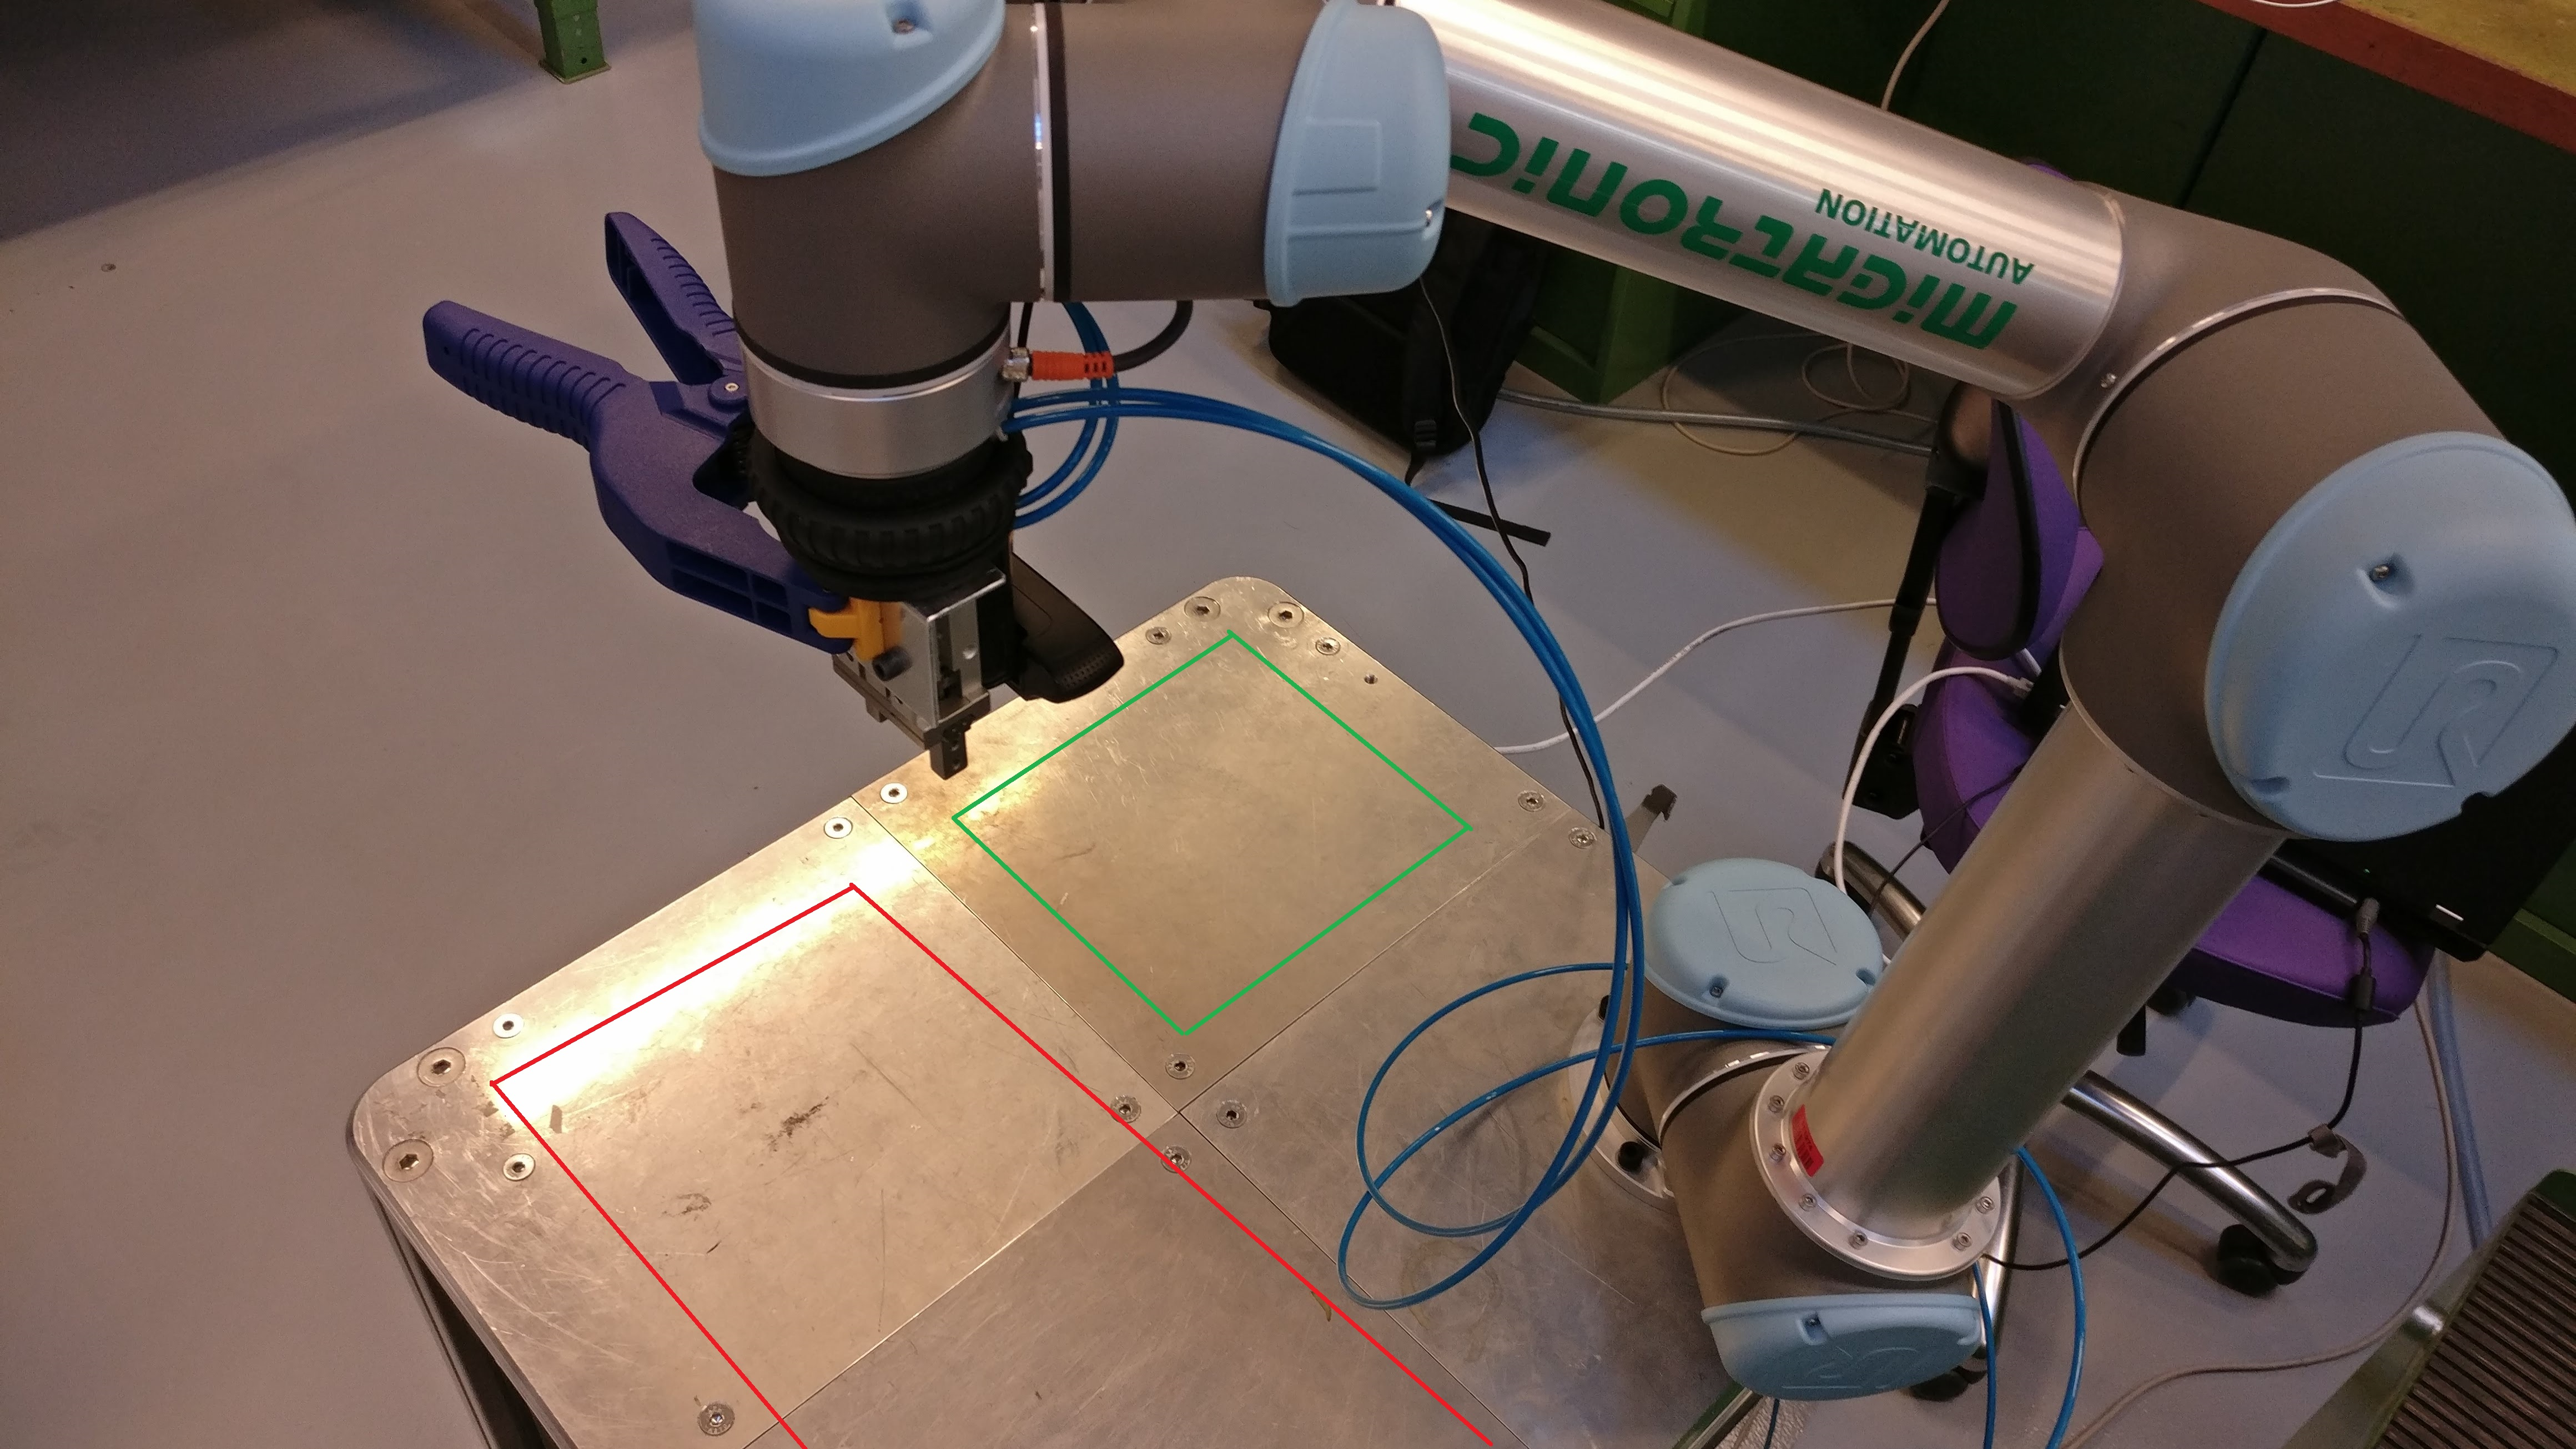
\includegraphics[width=\textwidth]{figures/workarea.jpg}
\caption{}
\label{fig:workarea}
\end{figure}

The camera was mounted to the tool, \autoref{fig:tool_cam}, as there were no other places to mount it. The benefits of this approach are that the camera does not obstruct the robot when it is moving. Another benefit is that the cameras frame is known when the tools is known, except it is flipped on one of the axis.

\begin{figure}[h]
\centering
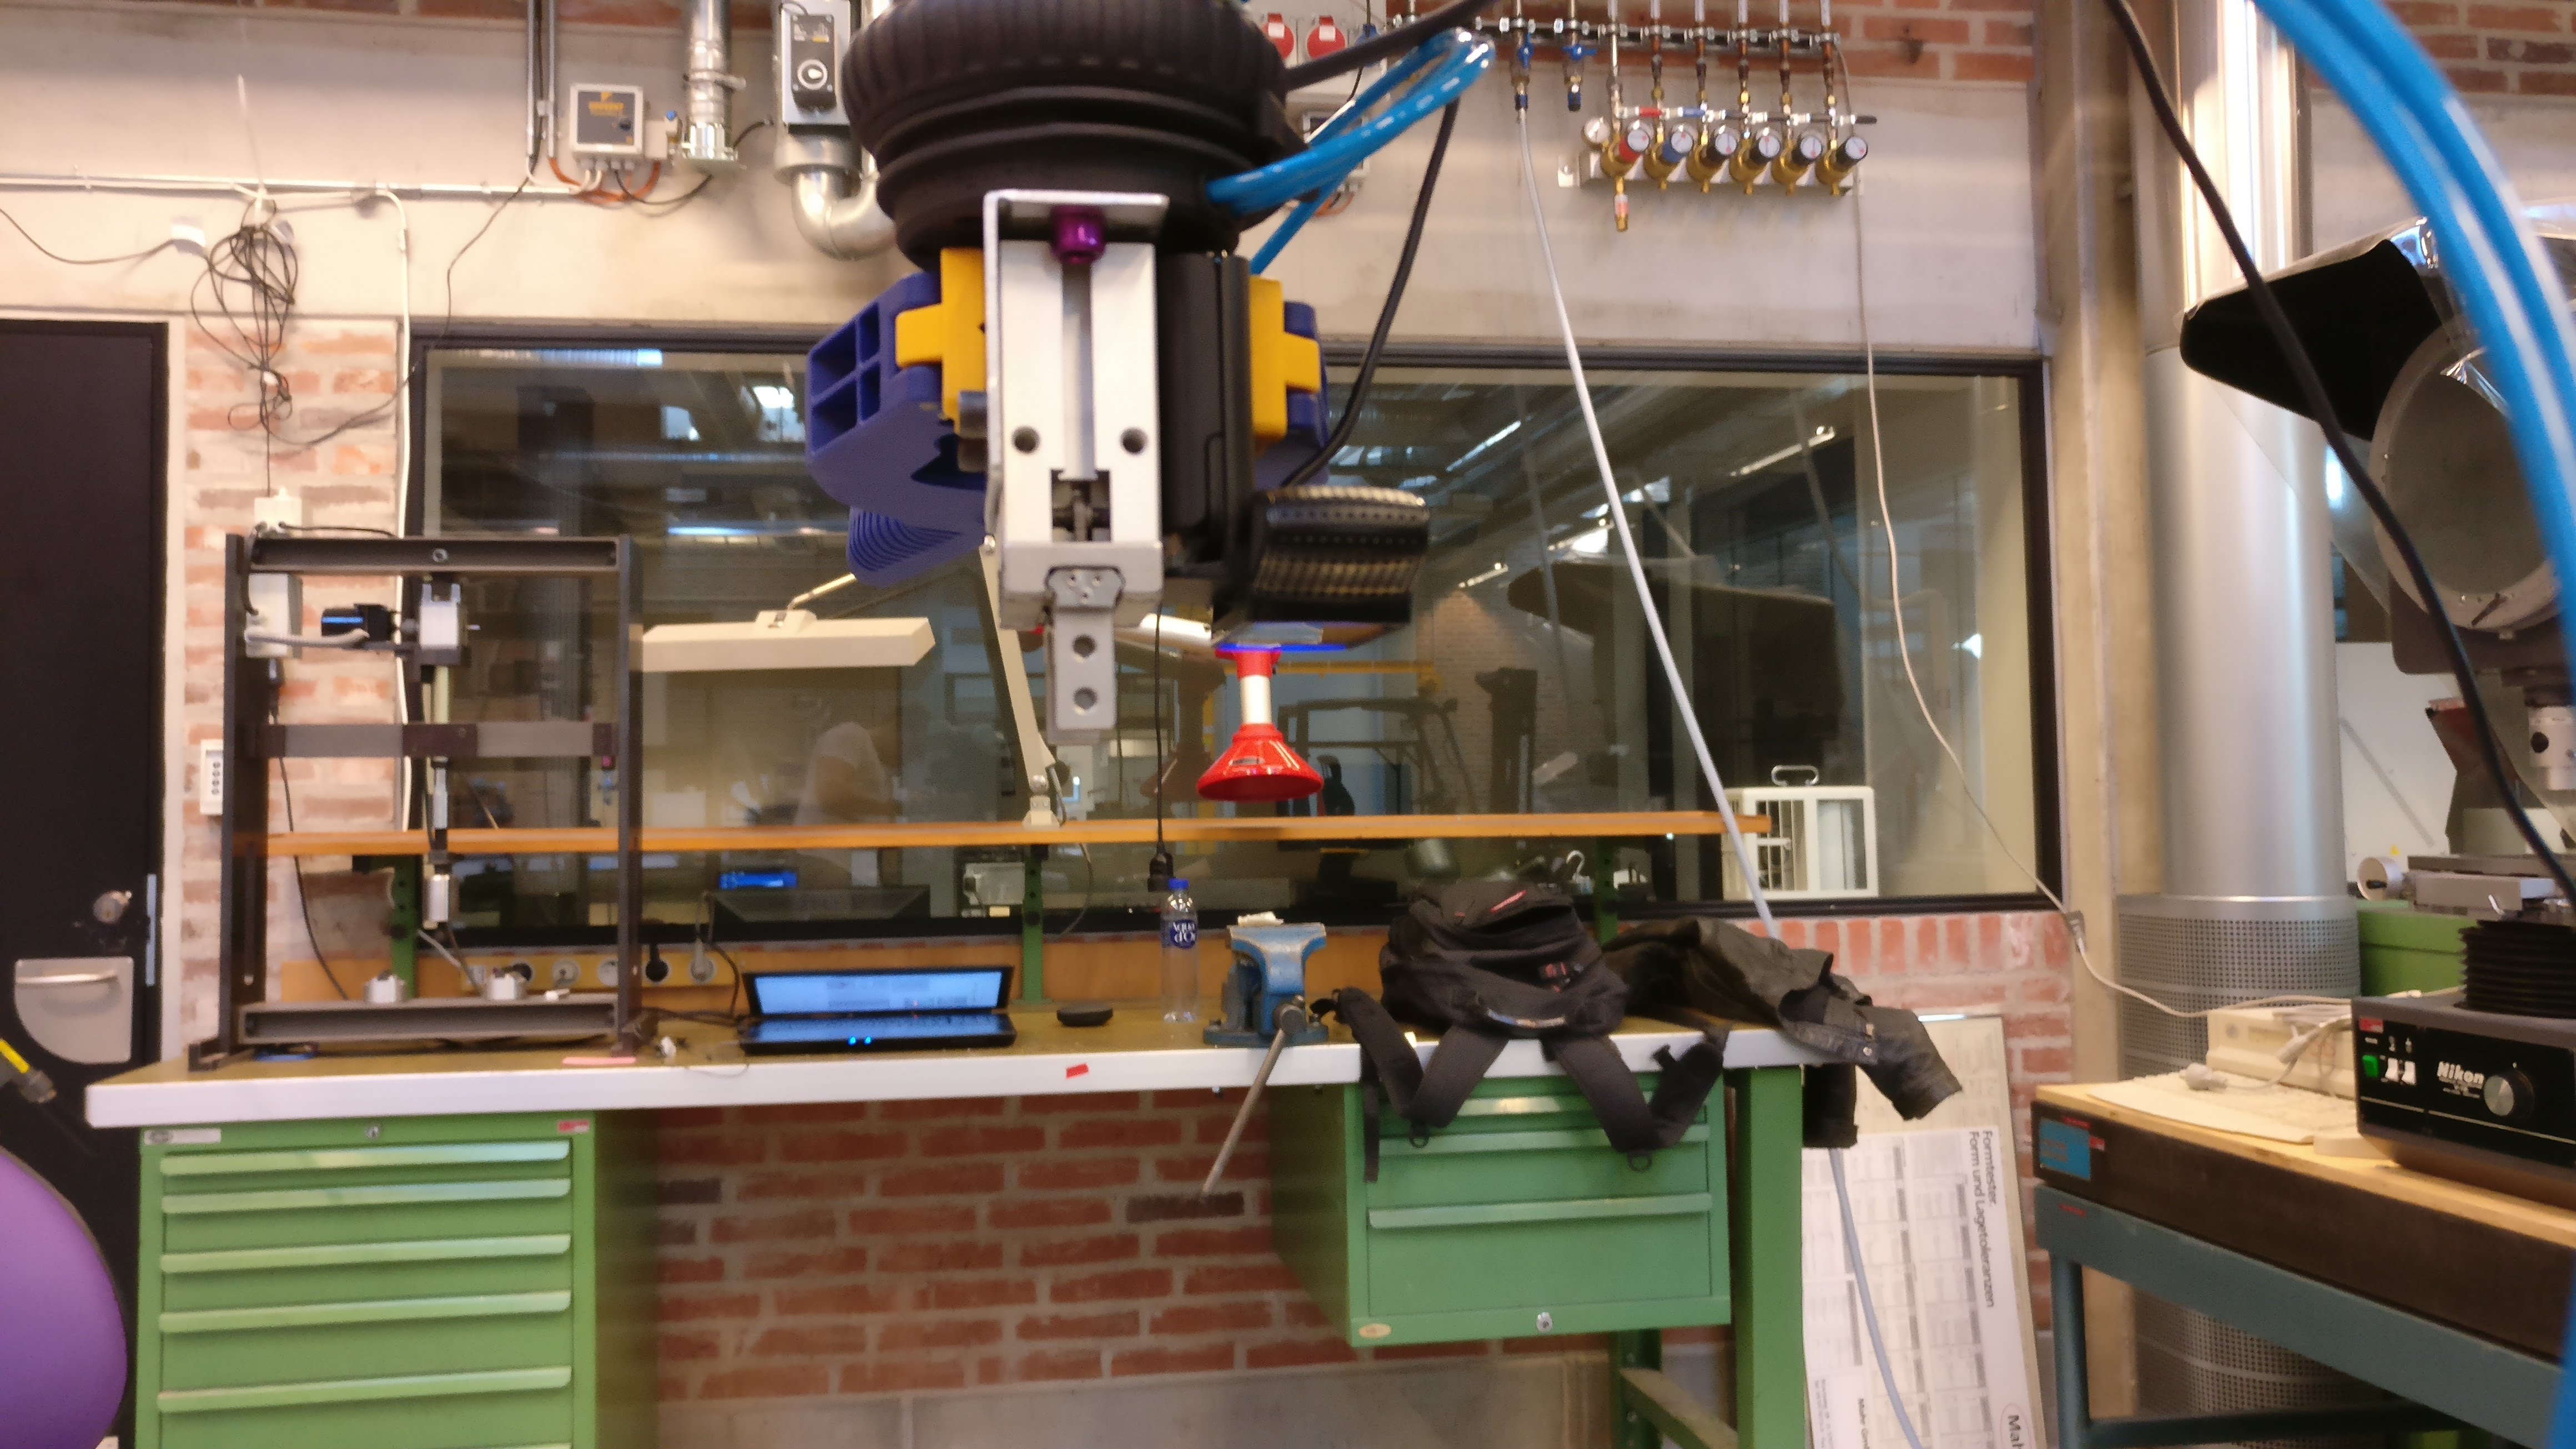
\includegraphics[width=\textwidth]{figures/tool_cam.jpg}
\caption{}
\label{fig:tool_cam}
\end{figure}
\chapter{Calibration}

\section{From image to camera}
\begin{figure}[h]
\centering
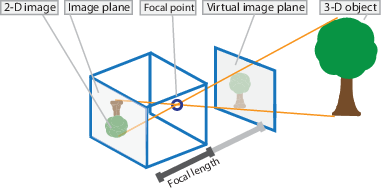
\includegraphics[width=\textwidth]{figures/camera_calibration_focal_point.png}
\caption{}
\label{fig:camera_calibration_focal_point}
\end{figure}
When taking an image for the use of detecting an object it is necessary to transform the image frame into the robot frame. First the image has to be transformed from world coordinates into camera coordinates and then to robot coordinates. When going from world to camera the pinhole camera model can be used. A graphical depiction of the model is shown in \autoref{fig:camera_calibration_focal_point}. The camera is assumed to be a box where no light can enter except from a small hole called the focal point. The light that is cast on the back wall is an inverted 2D representation of the 3D world outside of the box. The 2D image depends on the distance from the focal point to the back wall, called the focal length. The transformation is split into two parts; from world coordinates to camera coordinates and from camera coordinates to image coordinates. This is done by finding the intrinsic and extrinsic parameters. The intrinsic parameters look like shown in \autoref{eq:intr_param}.

\begin{equation}\label{eq:intr_param}
\begin{bmatrix}
u \\
v \\
w 
\end{bmatrix} 
 =
\begin{bmatrix}
a_x & s & x_0 & 0 \\
0 & a_y & y_0 & 0 \\
0 & 0 & 1 & 0 
\end{bmatrix}  
\begin{bmatrix}
x_s \\
y_s \\
z_s \\
0 
\end{bmatrix}
\end{equation}

where $x_s, ~y_s, ~z_s$ are the scene points in the camera coordinate system, $u, v, w$ are the homogeneous image coordinates where $w$ is a scaling factor. The parameters are $a_x, a_y$ which are the focal length. $x_0$ and $y_0$ are to translate the image centre to be the actual image centre since there may be an offset due to fabrication issues.  $s$ is the pixel skew parameter but it is usually set to 0.

The extrinsic parameters are a translation and rotation that describe where in the world the camera is located and how it is oriented. The parameters can be expressed as:
$ \begin{bmatrix}
R & -RC  \\
0_{3}^{T} & 1 
\end{bmatrix}  $
where $R$ is the rotational $3\times 3$ matrix and $-RC$ is the $3$dimensional vector translation. To get the whole transformation it would look like shown in \autoref{eq:cam_trans}.

\begin{equation}\label{eq:cam_trans}
\begin{bmatrix}
u \\
v \\
w 
\end{bmatrix} 
 =
\begin{bmatrix}
a_x & s & x_0 & 0 \\
0 & a_y & y_0 & 0 \\
0 & 0 & 1 & 0 
\end{bmatrix}  
\begin{bmatrix}
R & -RC  \\
0_{3}^{T} & 1 
\end{bmatrix}
\begin{bmatrix}
x_s \\
y_s \\
z_s \\
0 
\end{bmatrix}
\end{equation}

Lastly there can also be some radial distortion in the image caused by the lens, which causes lines that are linear in the world coordinate to appear non-linear in the image. This correction can be computed by using images with objects with known straight lines. To get all these parameters the Camera Calibration Toolbox for Matlab by Jean-Yves Bouguet can be used.  Here 10 to 20 images are taken of a checker board pattern as shown in \autoref{fig:checkerbord_pattern}, where the size of the squares is known, and from this it is possible to estimate the intrinsic and extrinsic parameters and distortion of the camera.

\begin{figure}[h]
\centering

\includegraphics[width=0.8\textwidth]{figures/checkerbord_pattern.png}
\caption{}
\label{fig:checkerbord_pattern}
\end{figure}


\section{From Image to Robot}
Once the parameters are known they need to be transformed into robot coordinates. For this the transformation matrix from the camera coordinates to robot is needed. A way to simplify this is to use a different approach than finding the camera parameters. If the camera is orthogonal to the planar space that the robot needs to operate in it can be assumed that image is simply a version of the planar space with constant scaling. If a point is known in pixel coordinates and in robot coordinates it is possible to compute a simple projection between the points. Then it is not necessary to get the camera parameters and know the robots frame as long as the mapping is known. The mapping can be found as shown in \autoref{fig:camera_robot_shortcut} with \autoref{eq:cam_calib1}.

\begin{equation}\label{eq:cam_calib1}
\begin{split}
x_{rob}&=\theta_{0}+\theta_{1}*x_{img}+\theta_{2}*y_{img}\\
x_{rob}&=(1+*x_{img}+y_{img}) * \vec{\theta}
\end{split}
\end{equation}

Where $x_{rob}$ is the $ x $ coordinate for the robot in a place in the image space. $x_{img}$ and $y_{img}$ are the pixel coordinates of the exact same point with $\theta_1$ and $\theta_2$ as scaling factors for when the robot moves in the $ x $ direction in robot coordinates how much does it move in $ x $ and $ y $ of the pixel coordinates. $\theta_0$ is the offset that comes from the robot's base not having the same origin as the image. When done for both $ x $ and $ y $ the result is found using \autoref{eq:cam_calib2}
 
\begin{equation}\label{eq:cam_calib}
\begin{split}
x_{rob}&=(1+*x_{img}+y_{img})*\vec{\theta}\\
y_{rob}&=(1+*x_{img}+y_{img}) * \vec{\phi}
\end{split}
\end{equation}

Where $\theta$ is the $ x $ parameters and $\phi$ is the $ y $ parameters. These can be solved for by using multiple known points and their accompanying robot and pixel coordinates like shown in \autoref{eq:rob_x}

\begin{equation}\label{eq:rob_pix}
\begin{bmatrix}
x_{rob1} \\
x_{rob2} \\
x_{rob3}
\end{bmatrix} 
 =
\begin{bmatrix}
1 & x_{img1} & y_{img1} \\
1 & x_{img2} & y_{img2} \\
1 & x_{img3} & y_{img3} 
\end{bmatrix}  
* \vec{\theta}
\end{equation}

To then go to robot coordinates from pixel coordinates \autoref{eq:rob_coord} is used.

\begin{equation}\label{eq:rob_coord}
\begin{bmatrix}
x_{rob} \\
y_{rob} \\
\end{bmatrix} 
= 
\begin{bmatrix}
1 & x_{img} & y_{img}\\
\end{bmatrix} 
\begin{bmatrix}
\theta_0 & \phi_0\\
\theta_1 & \phi_1\\
\theta_2 & \phi_3  
\end{bmatrix}  
\end{equation}

\begin{figure}[h]
\centering
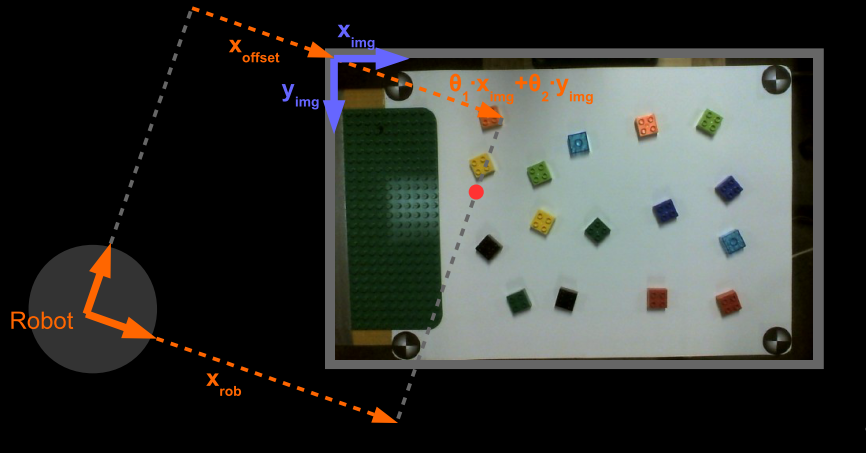
\includegraphics[width=\textwidth]{figures/camera_robot_shortcut.png}
\caption{}
\label{fig:camera_robot_shortcut}
\end{figure}

This procedure will increase in precision with the increasing number of points used. In the project it is chosen to use three stationary points in the workspace frame of the operating table.

\chapter{Computer Vision}\label{ch:img_proc}
The computer vision part is the image processing part of the project. Here the machine differentiates the different \lego bricks and their individual colours. Furthermore their pixel position is found to be converted to world coordinates later in the program.
This is done to let the robot use the knowledge of the different colours to automatically assemble the figures with the right coloured bricks.
To find the bricks in the picture, several steps are made to differentiate the colours:

\begin{itemize}
	\item Format conversion
	\item Background subtraction
	\item Colour thresholding
	\item Noise removal
	\item BLOB analysis
	\item Feature extraction
\end{itemize}

The original picture processed is shown in \autoref{fig:orig_pic}.

\begin{figure}
	\centering
	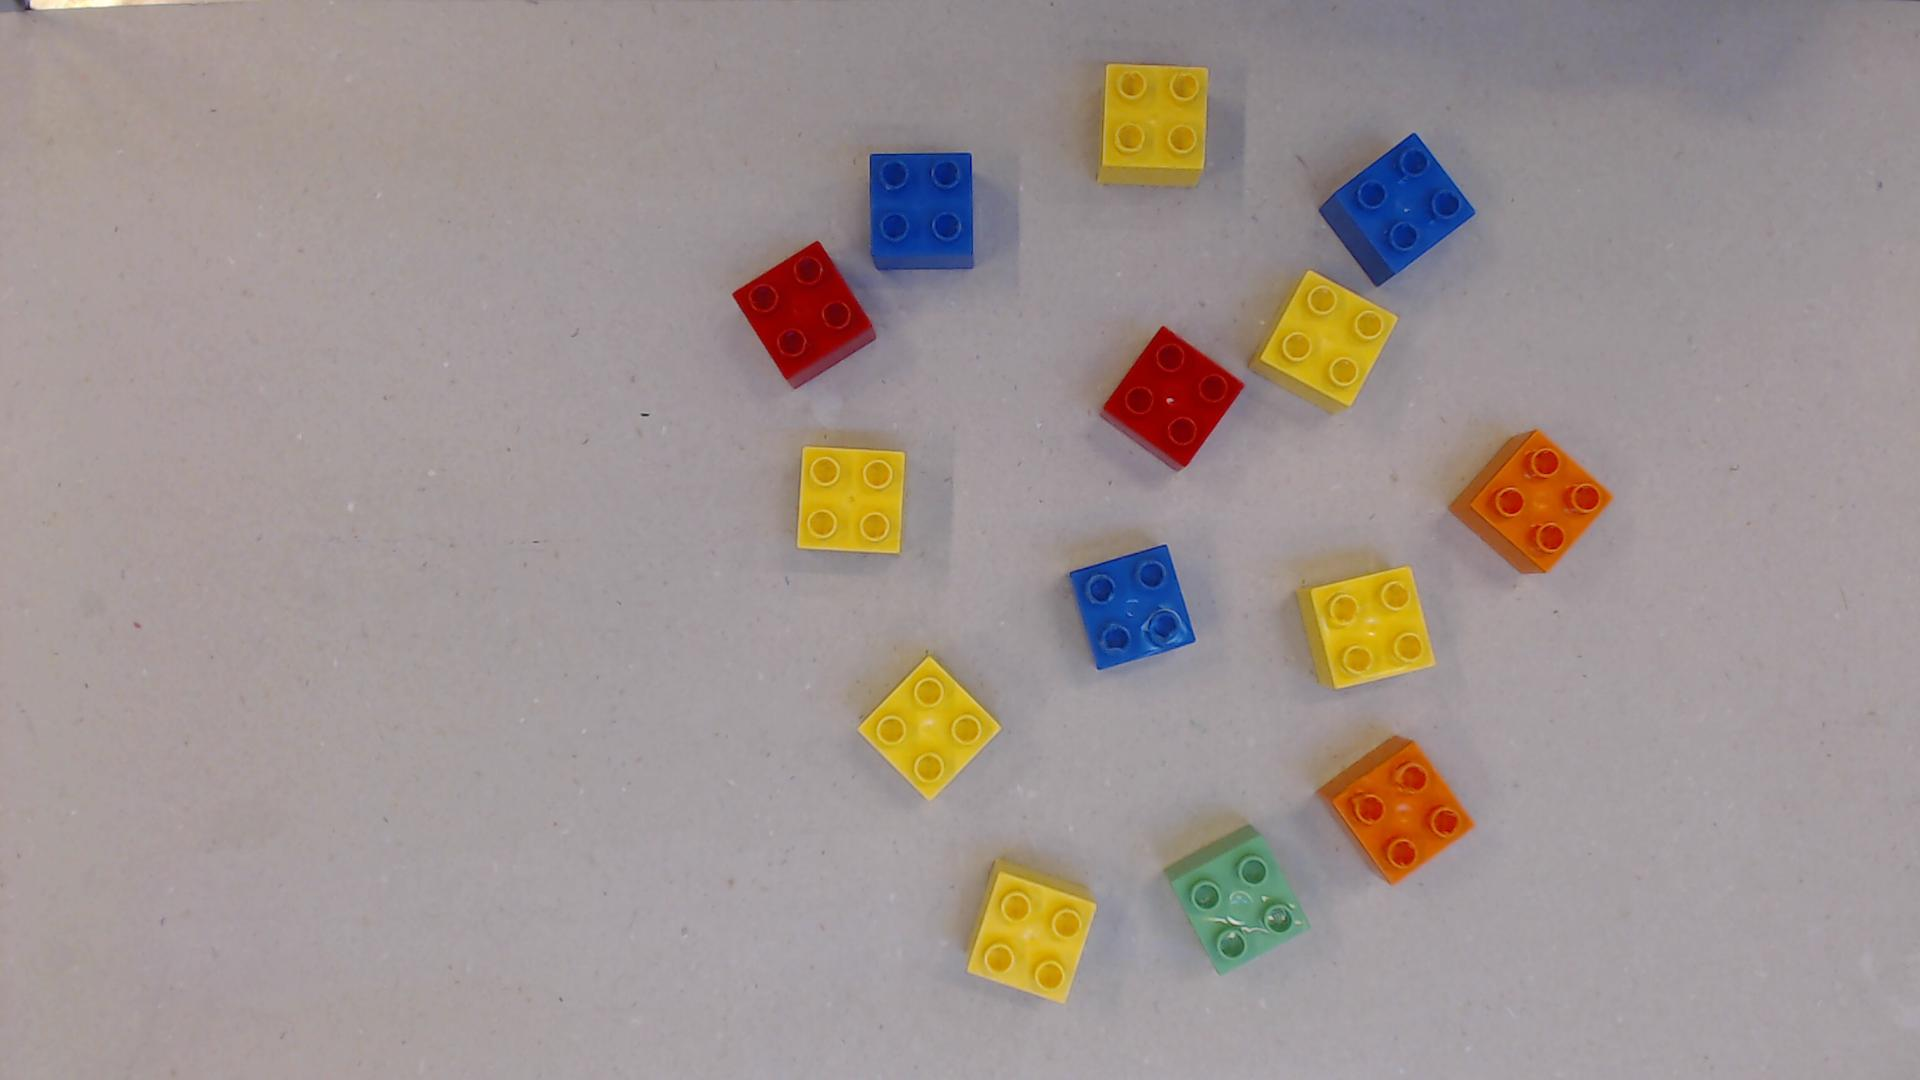
\includegraphics[width=0.69\textwidth]{figures/orig_pic.jpg}
	\caption{Original picture taken by the webcam attached to the robot.}
	\label{fig:orig_pic}
\end{figure}

\section{Format Conversion}
The original picture taken by the webcam is in RGB and is converted to a chromaticity image. This is done using \autoref{eq:rgb_to_rgi}:

\begin{equation}\label{eq:rgb_to_rgi}
	r=\frac{R}{R+G+B}, ~g=\frac{G}{R+G+B}, ~I=\frac{R+G+B}{3}
\end{equation}

Chromaticity is given from the chromaticity plane. This is shown in \autoref{fig:chrom_plane}. This is done since the colours are being normalised to avoid influence by illumination. Then the colour description is supplemented by an intensity as calculated in \autoref{eq:rgb_to_rgi}. This will be referred to as RGI and the conversion is RGB to RGI.


\begin{figure}[H]
	\centering
	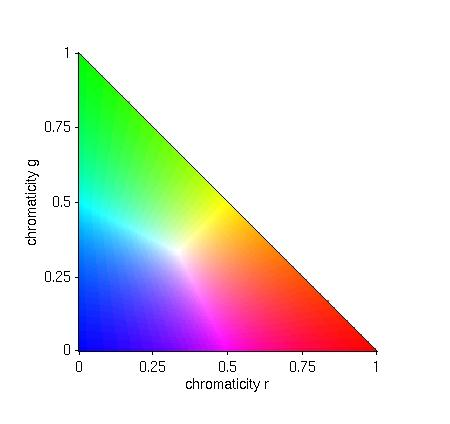
\includegraphics[width=0.7\textwidth]{figures/chrom_plane}
	\caption{Chromaticity plane}
	\label{fig:chrom_plane}
\end{figure}

The advantage of this is, that this should allow for colour thresholding on any image as it disregards illumination.

\section{Background Subtraction}
The background of the image is subtracted to ease the localisation of the brick edges. This is done by taking a picture of the surface without any bricks as a background image from the exact same position as the original image.
To avoid unwillingly removing any objects from the new image generated a threshold is set fro specific pixel values.

Firstly the RGB image of the background is converted to an RGI image. The subtraction is then performed pixel-wise using the formula shown in \autoref{eq:back_sub}. The subtraction is done using the two RGI images.

\begin{equation}\label{eq:back_sub}
	F(x,y) = I(x,y) - B(x,y)
\end{equation}

The thresholding is done by setting a threshold a value and doing a pixel-wise comparison. Should any of the channels have a higher value than the threshold, the pixel will be kept as a non-background pixel value.

\section{Colour Thresholding}
The colour thresholding is done to separate the individual brick colours from each other. The thresholding is done by comparing the pixel values of the RGI image to a set threshold for each channel. Firstly a threshold is applied to the intensity channel. This is done to rule out coloured pixels which may be indistinguishable because of too small an intensity. 

The colour thresholding is then made on the image. This is done for every brick colour used in the project by setting thresholds for both $r$ and $g$ channels to match the desired colour of a brick. A small pseudocode example is shown below:
\lstset{language=Pascal}
\begin{lstlisting}[frame=single]
if: 
	TH_r_min < r < TH_r_max AND
	TH_g_min < g < TH_g_max
then: object pixel
else: non-object pixel
\end{lstlisting}

If the pixel satisfies the set thresholds for the two channels, it is marked as a binary $1$ in an output image.

To set the thresholds fro the different colours in the $r$ and $g$ channels the RGI image is analysed. By cropping the picture to match each brick colour and analysing each for the chosen colour the thresholds are found by taking the $5\%$ and $95\%$ percentiles are found and used as the thresholds for each colour.

\section{Noise Removal}
The noise removal also known as morphology is done as the images generated from thresholding can contain some outliers which is not entire bricks but is recognised inside the threshold limits. Furthermore the bricks recognised contain some holes which is preferred to be filled.

To do this morphology the \textit{hit} and \textit{fit} operations are taken in use also known as dilation and erosion. These are firstly used to close the holes in the bricks and then opening to remove noise.
For this kernels for both dilation and erosion are defined. The functionality of both dilation and erosion is shown in \autoref{fig:dil_eros}

\begin{figure}
	\centering
	\begin{subfigure}[b]{0.45\textwidth}
		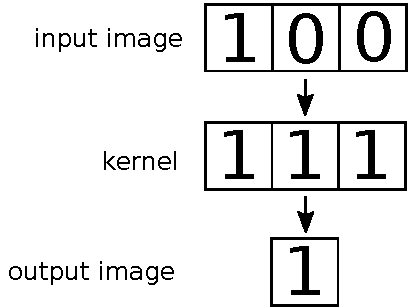
\includegraphics[width=\textwidth]{figures/dilation}
		\caption{Dilation kernel}
		\label{fig:dilation}
	\end{subfigure}
	\begin{subfigure}[b]{0.45\textwidth}
		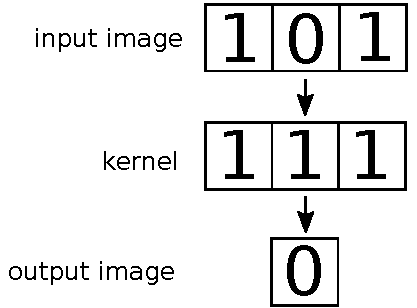
\includegraphics[width=\textwidth]{figures/erosion}
		\caption{Erosion kernel}
		\label{fig:erosion}
	\end{subfigure}
	\caption{Example of dilation and erosion kernel.}
	\label{fig:dil_eros}
\end{figure}

\section{BLOB Analysis}
The BLOB analysis is made to find the location of the bricks but also to find the rotation of the bricks to pick them up correctly. To do this a classification is necessary. This is done using the Grassfire algorithm with 4-connectivity. This enumerates each pixel belonging to a BLOB on the images for each of the brick colours.

The next step is finding the centre of the BLOBs or bricks, done by using centre of mass. This is calculated using the formulas shown in \autoref{eq:mass_centre}.

\begin{equation}\label{eq:mass_centre}
	x_m = \frac{1}{N}\sum_{i \in object}x_i, ~y_m= \frac{1}{N}\sum_{i \in object}y_i 
\end{equation}


To be able to pick up the bricks properly, the rotation of the bricks must be found. By calculating the distance from each pixel, forming a BLOB of a brick, to the centre of the BLOB the four corners are found by finding the four pixels furthest away from the centre. By defining four vectors from the centre of the brick to each corner the angles are calculated and by that the rotation. This is found by finding the mean of the four angles. In illustration of the vectors defined of the BLOB is shown in \autoref{fig:rot_fig}.

\begin{figure}[H]
	\centering
	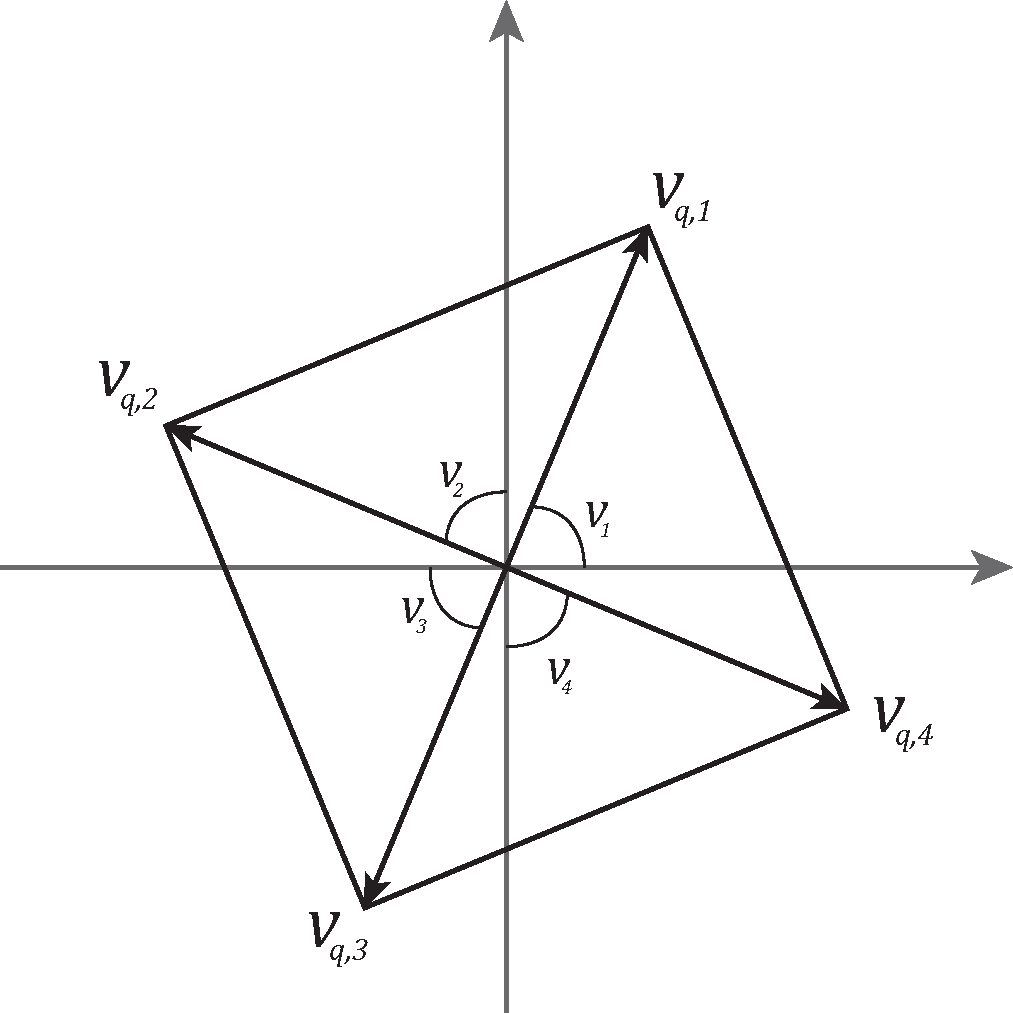
\includegraphics[width=0.65\textwidth]{figures/rot_fig}
	\caption{Rotations found from vectors and corners in a BLOB}
	\label{fig:rot_fig}
\end{figure}

The final result of the computer vision part yields five arrays with brick information of each colour and brick. This includes position and rotation used to locate and pick up the bricks. A final informational image of this including a directional vector showing the rotation is shown in \autoref{fig:fin_pic}.

\begin{figure}[H]
	\centering
	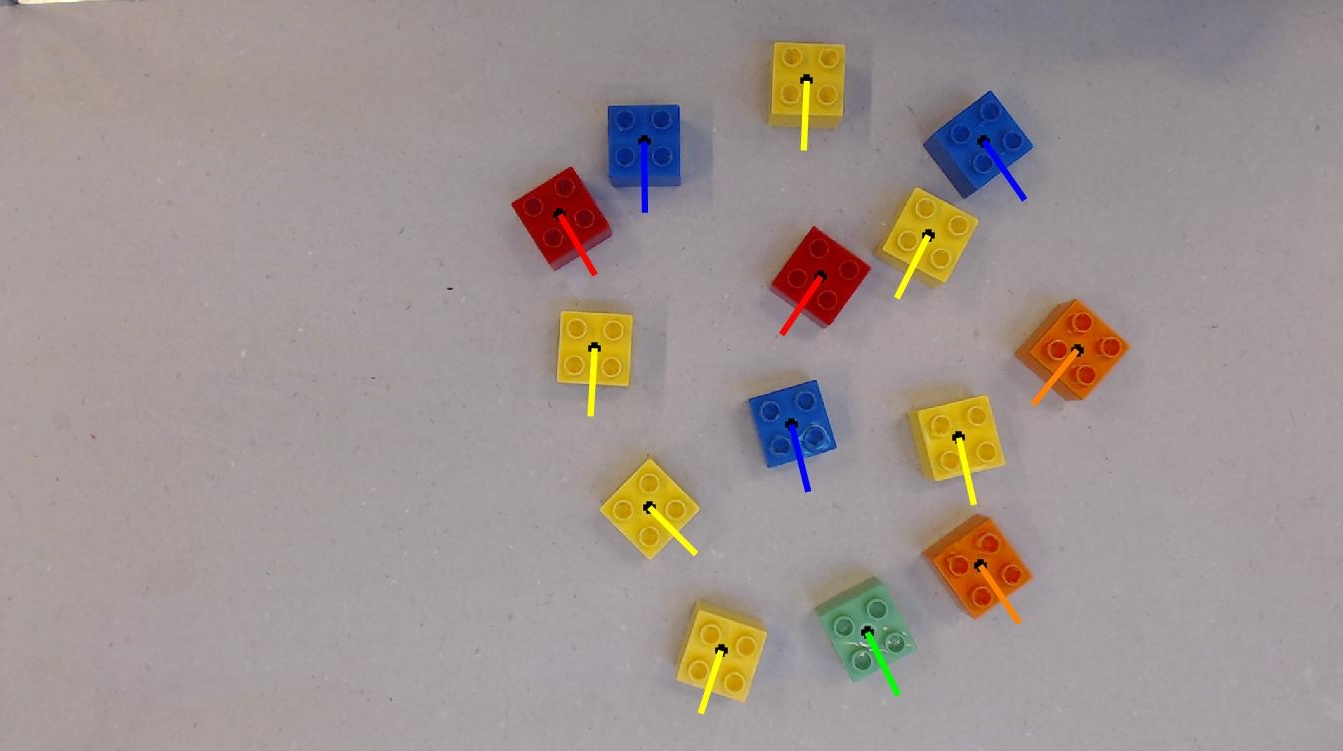
\includegraphics[width=\textwidth]{figures/fin_pic.jpg}
	\caption{Final informational image including brick centre and rotation directional vector.}
	\label{fig:fin_pic}
\end{figure}
\chapter{Assembly}
\section{Robot Control}
The robot was controlled by using a Matlab script that creates an interface to the UR robot. This is done with a TCP/IP connection. The robot is then controlled linearly or by joint values. Since the location of the brick is known, inverse kinematics can be used get the robot to that location.  As long as the location and orientation of where the end effector is supposed to be, the internal software of the robot takes care of the inverse kinematics.

\section{Final assembly}
%When actually performing it in practice this is how we did it. First the hand eye calibration was run. The points chosen for calibration were the bolts that were in the workspace because they were constant points. The robot tool was then placed horizontal to the workspace using the teach pendant so the bolt was in the centre of the gripper. The tool's x and y positions were then saved for calibration. Since these positions would not change as the workspace was where the robot was mounted it was not necessary to get more than once. The the same pixel values of the same location was found and the calibration was done.  
%
%After the calibration a brown flat cardboard was put onto the workspace to minimize the reflection from the metallic surface. Then an image of the workspace is taken without the bricks and with the bricks for background subtraction. Then the image processing is done resulting in brick centres, colours and rotations. The robot can now be ordered to assemble a figure e.g. Homer by taking the first appropriate bricks from the top of the image. It moves to the centre of the brick's position an rotates the corresponding degrees around the Z axis to be able to grab the brick.  The figure is then delivered to the drop off zone and prepares for a new order. 
%

The assembly is made on the platform where the Universal Robot (UR5) is mounted. Here a piece of cardboard is laid out on the platform to occlude the shiny metal background, easing the image processing as this will give a plain background to process instead of a reflective surface.

For each initialisation of the program a new picture is taken of the background, then bricks are placed in the workspace and a picture is taken. The positions and orientation of the bricks are found using the image processing described in \autoref{ch:img_proc}.

When the image processing is done it is possible to order any of the five Simpsons characters from the MATLAB command window. Because of functionality issues with the gripper on the robot it was not possible to physically assemble the figurines. Instead the robot marks the two or three bricks used for the specific character, taking the theoretically height into account as well and moves to the drop-off point. A red brick was used as the middle piece in the Homer character as there was not any white bricks available. The amount of bricks was limited to the option of building one of each character. Had there not been any issues with the gripper the characters could have been assembled and placed in the drop-off area, as proved in the example video.




% For use if report is split up in parts
\bookmarksetup{startatroot}% Goto root of Table of Contents
\addtocontents{toc}{\bigskip}% Add space before next item in Table of Contents

% Appearance of the bibliography
\iflanguage{english}{%
\bibliographystyle{setup/plainnat_en}%
}{%
\bibliographystyle{setup/plainnat_dk}%
}
\label{LastPage}


%\bibliography{bib/VGIS8.bib}
%\label{bib:mybiblio}




%\setlength{\chapnumb}{2cm} % Ændrer længden på stregen under kapiteloverskriften så den passer til bilag
%\appendix % Start of appendix
%\addtocontents{toc}{\protect\setcounter{tocdepth}{0}} 


\end{document}
